%%%%%%%%%%%%%%%%%%%%%%%%%%%%%%%%%%%%%%%%%
% Simple Sectioned Essay Template
% LaTeX Template
%
% This template has been downloaded from:
% http://www.latextemplates.com
%
% Note:
% The \lipsum[#] commands throughout this template generate dummy text
% to fill the template out. These commands should all be removed when 
% writing essay content.
%
%%%%%%%%%%%%%%%%%%%%%%%%%%%%%%%%%%%%%%%%%

%----------------------------------------------------------------------------------------
%	PACKAGES AND OTHER DOCUMENT CONFIGURATIONS
%----------------------------------------------------------------------------------------

\documentclass[12pt]{article} % Default font size is 12pt, it can be changed here

\usepackage{geometry} % Required to change the page size to A4
\geometry{a4paper} % Set the page size to be A4 as opposed to the default US Letter

\usepackage{graphicx} % Required for including pictures

\usepackage{float} % Allows putting an [H] in \begin{figure} to specify the exact location of the figure
\usepackage{wrapfig} % Allows in-line images such as the example fish picture

\usepackage{lipsum} % Used for inserting dummy 'Lorem ipsum' text into the template

\linespread{1.2} % Line spacing

%\setlength\parindent{0pt} % Uncomment to remove all indentation from paragraphs

\graphicspath{{Pictures/}} % Specifies the directory where pictures are stored

\begin{document}

%----------------------------------------------------------------------------------------
%	TITLE PAGE
%----------------------------------------------------------------------------------------

\begin{titlepage}

\newcommand{\HRule}{\rule{\linewidth}{0.5mm}} % Defines a new command for the horizontal lines, change thickness here

\center % Center everything on the page

\textsc{\LARGE Sun-Yet-Sun University}\\[1.5cm] % Name of your university/college
\textsc{\Large Introduction to IT Systems Management}\\[0.5cm] % Major heading such as course name
\textsc{\large Fuzzy Learning Model}\\[0.5cm] % Minor heading such as course title

\HRule \\[0.4cm]
{ \bfseries The Thought of Implementing Fuzzy Learning in Recognizing Numerical Characters}\\[0.4cm] % Title of your document
\HRule \\[1.5cm]

\begin{minipage}{0.4\textwidth}
\begin{flushleft} \large
\emph{Author:}\\
Luo \textsc{Wei Qiang} % Your name
\end{flushleft}
\end{minipage}
~
\begin{minipage}{0.4\textwidth}
\begin{flushright} \large
\emph{Supervisor:} \\
Dr. Richard \textsc{Tor} % Supervisor's Name
\end{flushright}
\end{minipage}\\[4cm]

{\large \today}\\[3cm] % Date, change the \today to a set date if you want to be precise

%\includegraphics{Logo}\\[1cm] % Include a department/university logo - this will require the graphicx package

\vfill % Fill the rest of the page with whitespace

\end{titlepage}

%----------------------------------------------------------------------------------------
%	TABLE OF CONTENTS
%----------------------------------------------------------------------------------------

\tableofcontents % Include a table of contents


\newpage
%----------------------------------------------------------------------------------------
%	INTRODUCTION
%----------------------------------------------------------------------------------------

\section{Introduction} % Major section

Here we will talk about a thought of using fuzzy learning system in numerical character recognizing. The common way of doing OCR with neural network will be discussed, in which we will the role playing of fuzzy learning used in this method. Then we will discuss why fuzzy learning was chosen and why was that the fuzzy learning algorithm would not be implemented in all its process. In the third part, we will discuss the thought of implementing the fuzzy learning system into numerical ORC and at last we will talk about our future work.

%------------------------------------------------

\subsection{Fuzzy Learning} % Sub-section

Fuzzy learning is a type of learning that are to be used in uncertain or approximate reasoning. Which is to say, though the reasoning of the logic can be unclear, but this learning still requires some basic knowledge of the problem. \\
The other feature of fuzzy learning is that it allows a continuous transition of the determination rather than an abrupt change.
The features determined its role playing in OCR.

%------------------------------------------------

\subsection{BP neural Network} % Sub-section
BP neural Network is a well around learning method of approaching the answers to the problems. The core of BP neural network is using multiple layers to approach the true value of the reality. Within each layers, the difference between the results from the network and the true value get closer and closer.

%------------------------------------------------

\subsection{numerical OCR} 
The main task of numerical OCR is to recognizing the number in a picture. Each picture was size 20 * 20, which is to say that the picture contains 400 pixels to represent a number. The numbers various from 0 to 9. The pictures came from the machine learning course ml\_003.

%----------------------------------------------------------------------------------------
%	MAJOR SECTION 1
%----------------------------------------------------------------------------------------

\section{Recent Achievements} % Major section
\subsection{Achievement of Fuzzy Learning}
\subsubsection{General Achievement of Fuzzy Learning}
Fuzzy Learning had been used in various of recognizing problems. Most of which were control problems, pattern recognition problems, quantitative analysis problems, inference and information retrieval problems. \\
In Toshinori Munakata and Yashvant Jani's paper, the fields that had using fuzzy learning were well catagorized into several section. The various of the fields proves that fuzzy learning was a powerful algorithm.
\subsubsection{Achievement of Fuzzy Learning in OCR}
Several achievements of using fuzzy learning into OCR. Most of which are using it to recognizing the fonts and words that are natively designed with a line cross all the characters. \\
Utpal Garain and Bidyut B. Chaudhuri in 2002 present a way of doing OCRs in Devnagari and Bangla, which are two language and their scipts are like those below.
\begin{figure}[!htb]
    \begin{center}
        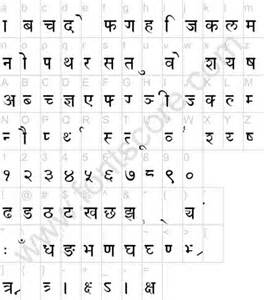
\includegraphics[width=0.38\textwidth]{devnagari}
        \mbox{    }
        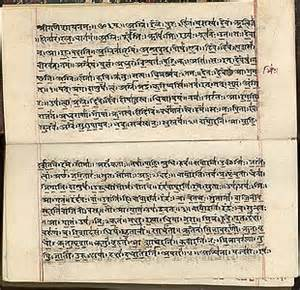
\includegraphics[width=0.38\textwidth]{devnagariPrinted}
    \end{center}
    \caption{Devnagari}
    \label{Devenagari}
\end{figure}
In their work, fuzzy system was used to cut the characters alone. As you can see in the previous pictures, this type of characters were sometimes combined together with some lines. A main task here was to separate them.
Ragjuraj Singh, C.S.Yadav, Prabhat Verma, Vibhash Yadav in 2010 present a paper also include fuzzy system in their OCR of Devnagari. The same choice of them were to use fuzzy system to recognize the cut position of this character and use ANN(Artificial neural Network) to identify each of these characters.


%----------------------------------------------------------------------------------------
%	MAJOR SECTION X - TEMPLATE - UNCOMMENT AND FILL IN
%----------------------------------------------------------------------------------------

\section{The Role Playing of Fuzzy Learning in OCR}
There are very few OCR learning algorithm using fuzzy learning. The reason of which is that fuzzy learning requires much pre-knowledge before implementing it to solve a real problem. In the analysis of OCR, it's not easy to extracting features from a set of pixels. As the input, if the original data are only pixels, it's very difficult to use fuzzy learning because the pixels, if were not processed before, rarely represent anything of the image (character). Something should be done to analyse the features of the origin pixels. \\
\begin{figure}[!htb]
    \begin{center}
        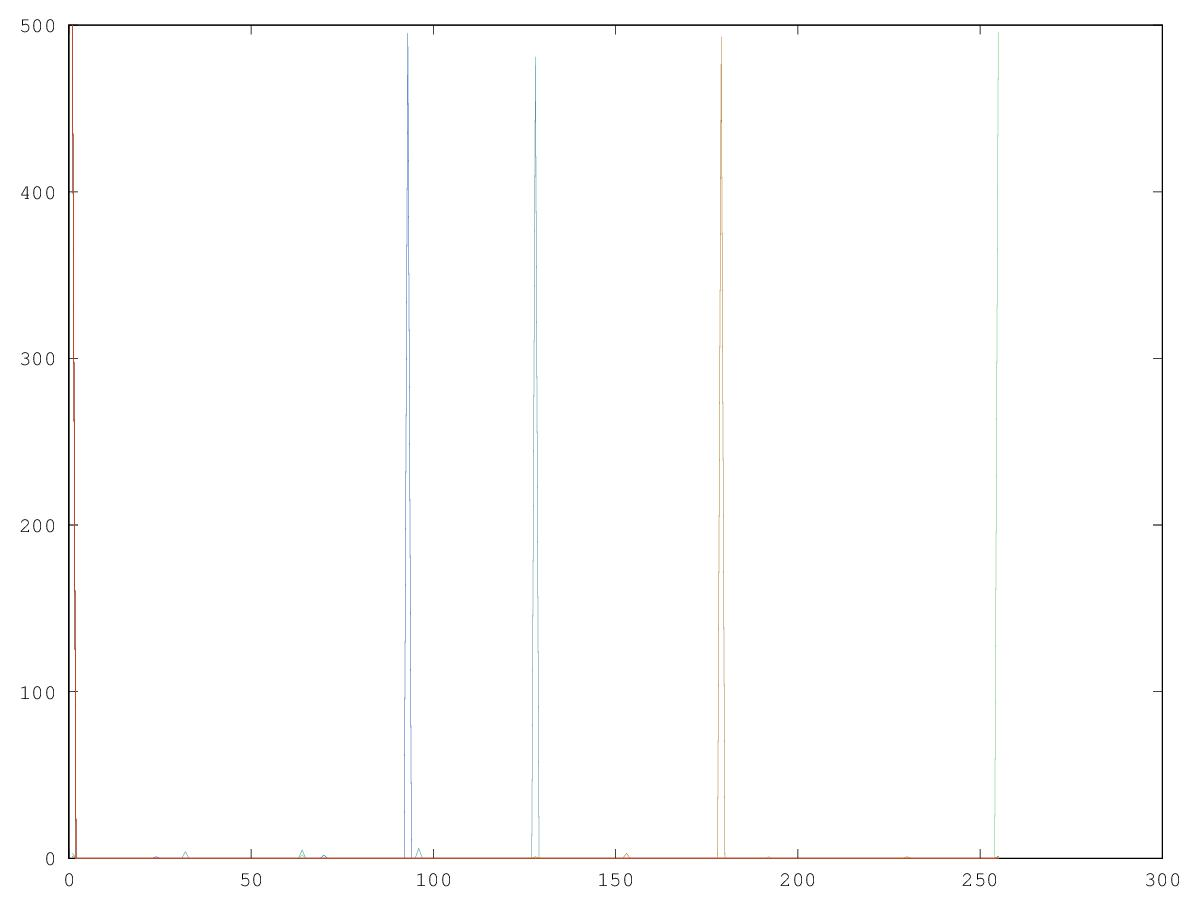
\includegraphics[width=0.38\textwidth]{25}
        \mbox{    }
        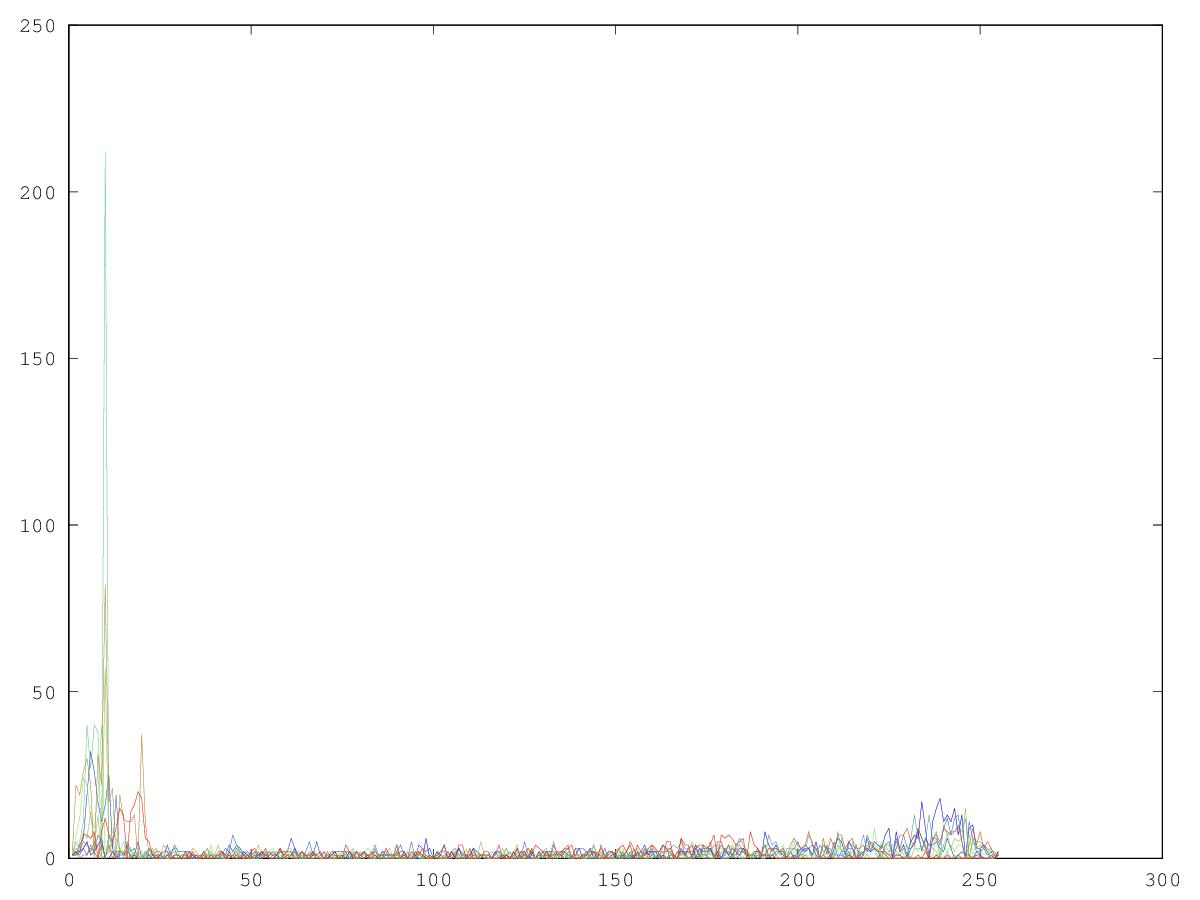
\includegraphics[width=0.38\textwidth]{225}
    \end{center}
    \caption{The frequency of numbers}
    \label{The frequency of numbers}
\end{figure}
The figures here depict the frequency of the number. The left one was the 25th pixel and the other one was the 225th pixel. Different color represent different numerical character. The X-axis represents the exact data of the numerical character and the Y-axis represents the amount of the numbers. From these two figures, we can clearly saw that clearly there were some features that were shown in the origin data. But that didn't have any actual meaning of the character. \\ 
Moreover, BP neural Network can easily classifying the numerical characters, and other characters without knowing the actual meaning of each pixels, and also, many other methods can be done in a high accuracy when the characters are separated. And so, fuzzy learning was rarely used in OCR. In Utpal G and Bidyut B.C's work, fuzzy learning was used to separate the characters. \\
\subsection{Details of previous design of Fuzzy System in OCR}
Most of the previous work use fuzzy system to separate the characters. In Utpal G and Bidyut B.C's work, they measure these factors to be used in fuzzy system.
\begin{itemize}
\item[\textbullet] The combine shapes of touching characters, using to identify the touching characters. 
\item[\textbullet] The ratio of the width and the height of the touching character. It's used to identify the touching characters.
\item[\textbullet] The vertical crossing count(number of transitions from white to black) for each pixel columns. This factor was used to find the cut position.
\item[\textbullet] The blob thickness. That related to the number of black pixels encountered in one column scan and the height of the character(From the highest black position to the lowest black position). This was used to find the cut position.
\item[\textbullet] The degree of middleness. The height of the character divides the total height of a character picture. Using to find the cut position. This was used to find the cut position.
\end{itemize}
At last, it was only used to identify whether they are touch characters and find the cut position.
\section{The thought of implementing fuzzy learning into numerical OCR}
The meaning of the word "thought" is that I didn't finish the learning system. Here are the design of the fuzzy system, which I will show the finished part and the un-finished part. \\
Our training data were the number pictures below:
\begin{figure}[!htb]
    \begin{center}
        
\includegraphics[width=0.38\textwidth]{example}
    \end{center}
    \caption{100 example numbers}
    \label{100 example numbers}
\end{figure}
To complete the learning system, we need to find the related factors from the input data, the pixels. There are a lot of options for us to do. \\
\subsection{Handling the input}
\begin{itemize}
\item[\textbullet] Firstly we could use the origin pixels to be the input. Suppose the membership function is M, then each pixel can have a hypothesis value. From the histogram we can see that some pixels can be used to identify the number. 
    \begin{figure}[!htb]
        \begin{center}
            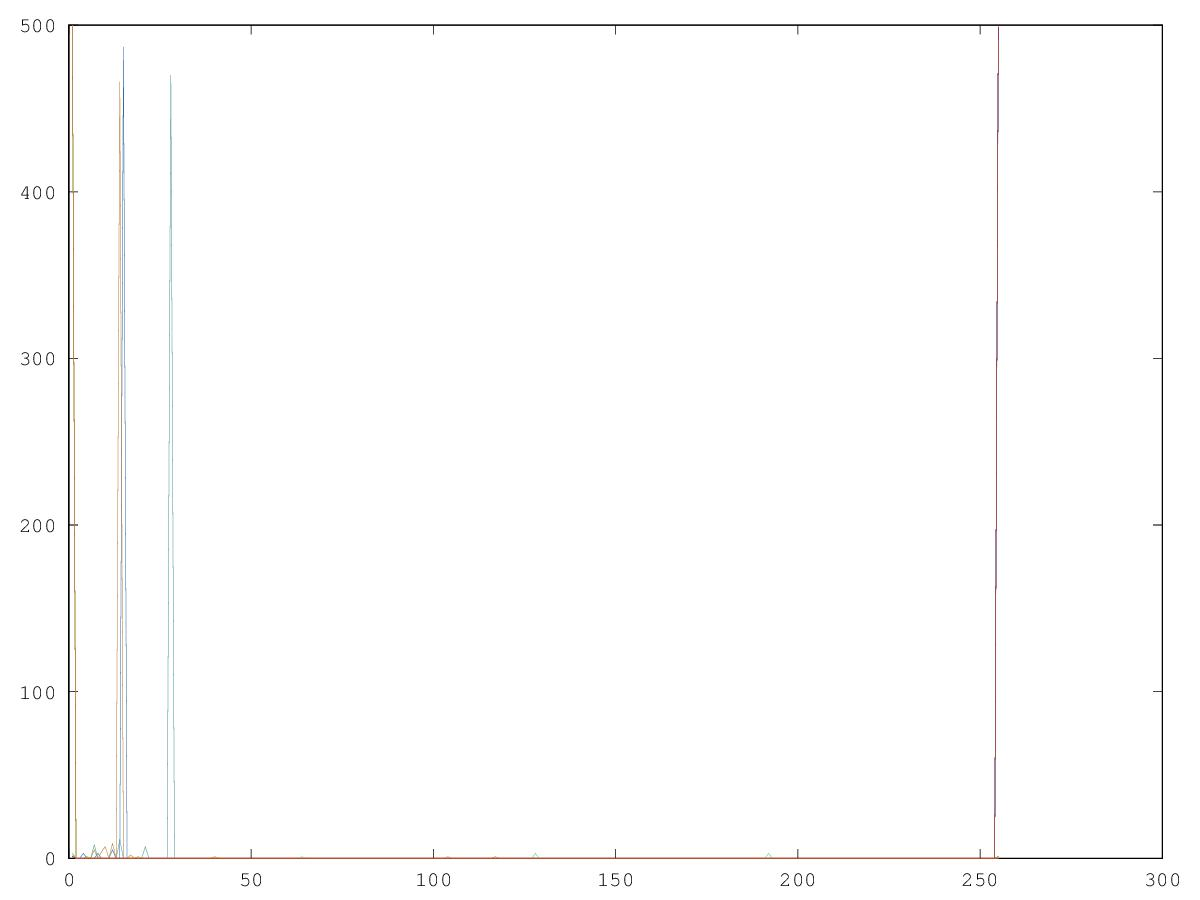
\includegraphics[width=0.38\textwidth]{26}
            \mbox{    }
            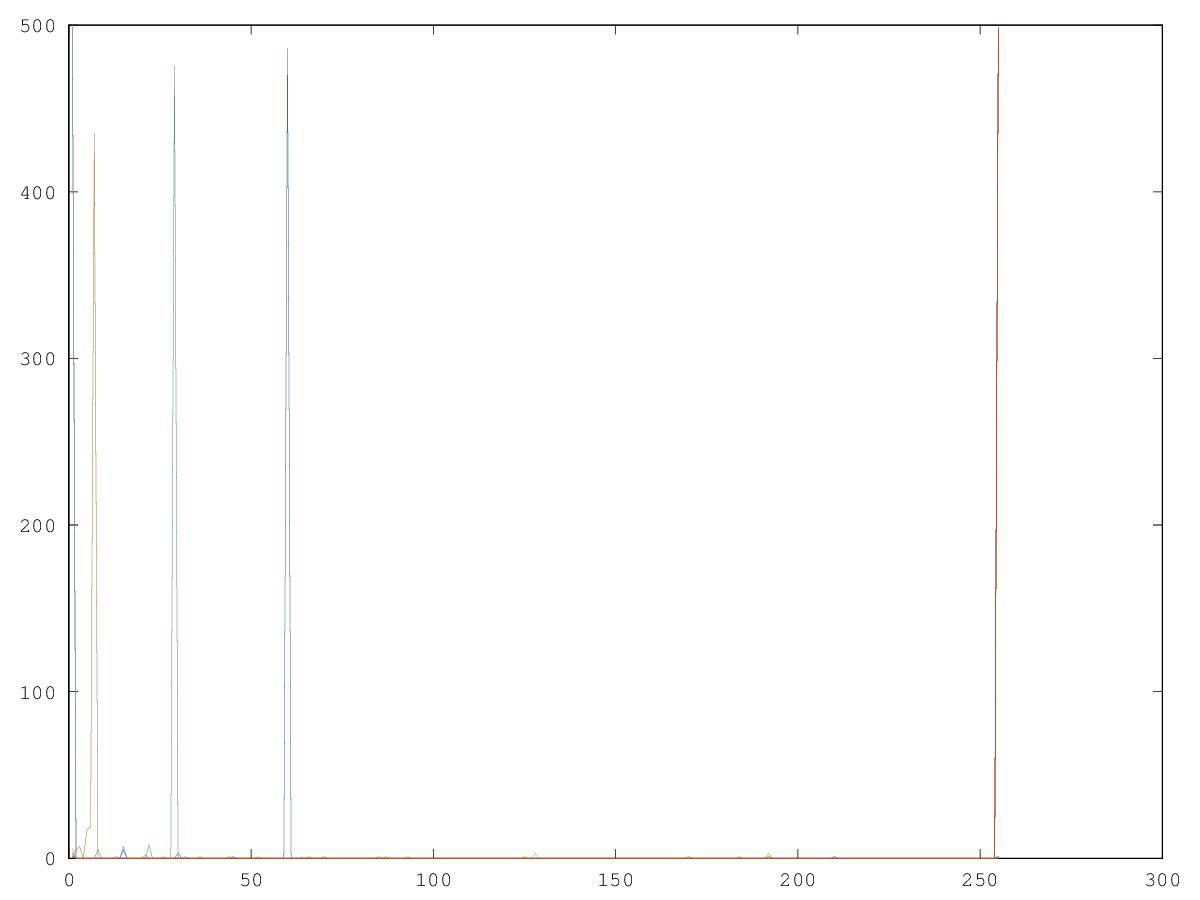
\includegraphics[width=0.38\textwidth]{27}
            \mbox{    }
            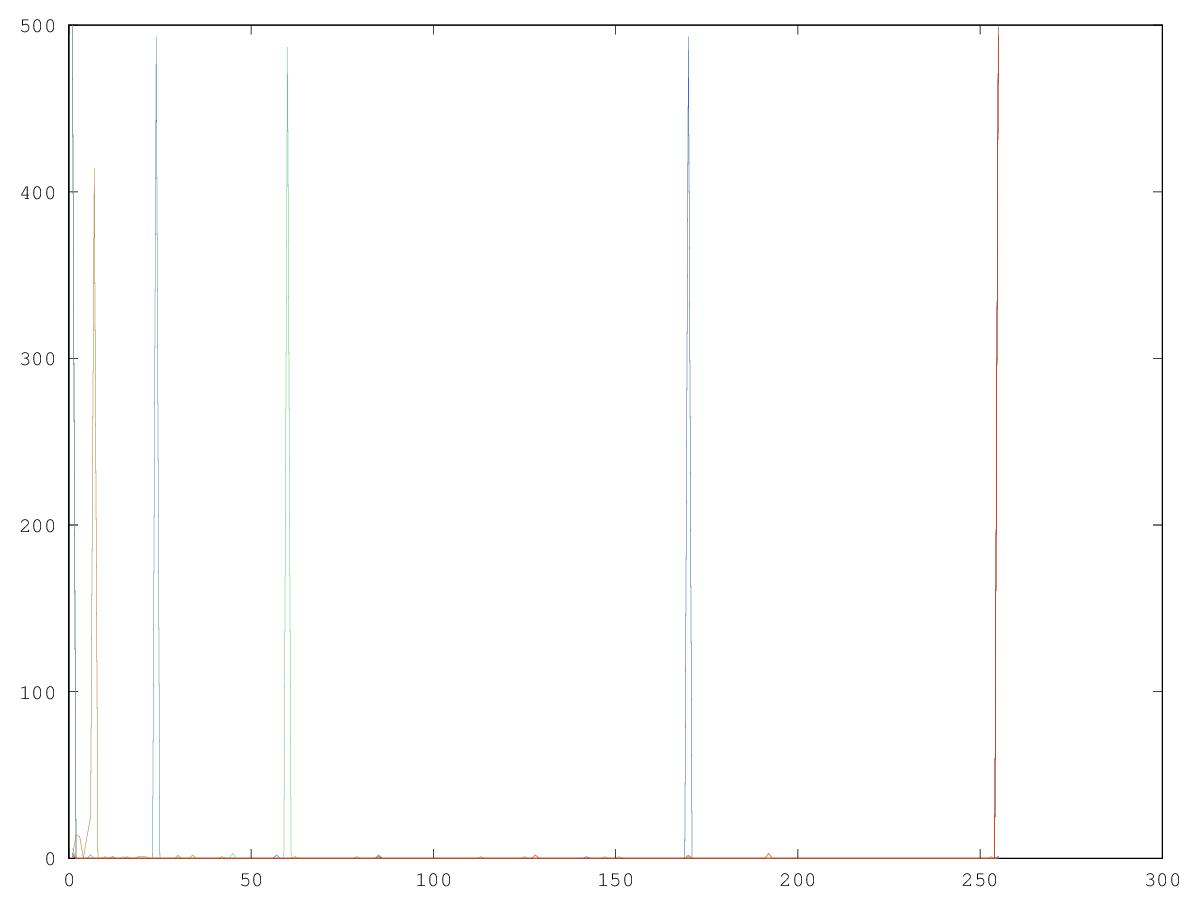
\includegraphics[width=0.38\textwidth]{28}
            \mbox{    }
            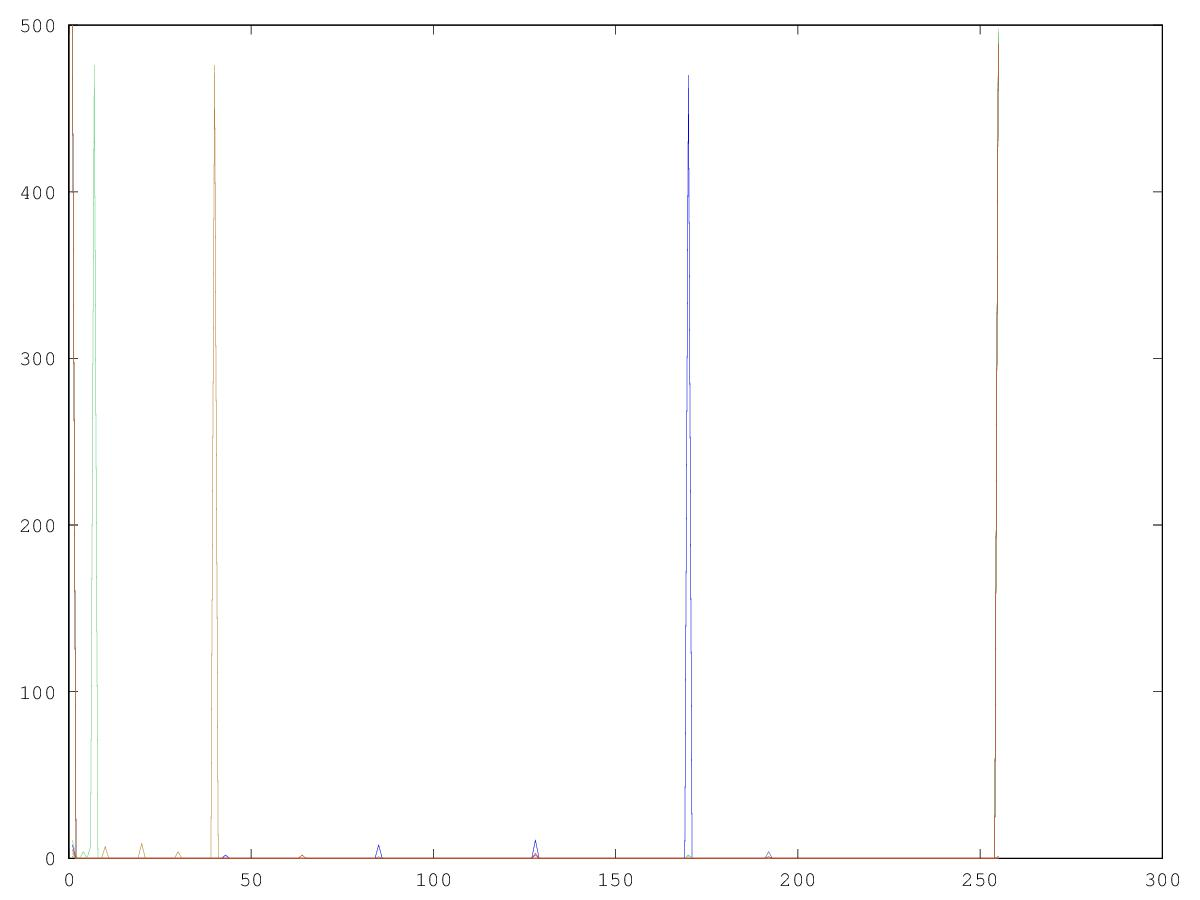
\includegraphics[width=0.38\textwidth]{31}
            \mbox{    }
        \end{center}
        \caption{The frequency of the 26th, 27th, 28th and the 30th number}
        \label{The frequency of the 26th, 27th, 28th and the 30th number}
    \end{figure}
    Thus, the origin data could probably be the suitable input for selecting the number.
\item[\textbullet] Aside from the pure pixel value, we can extract some higher level of information from each pictures. Here's are some aspects for the numerical recognition.
    \begin{itemize}
        \item The number of circles in one picture. In the numerical characters, there may have circles in a number. For example, '0' has a circle, and '1' has no circles. 
        \item The number of peaks in one picture. In the numerical characters, there may have some peaks in a number. For example, '0' has no peaks while '1' has at least 2 peaks.
        \item The center point of the picture of all the not-background pixels.
    \end{itemize}
\end{itemize}
The main task of selecting the form of input here are only to maximize the difference that enhance the learning system. 

\subsection{Handling the result value}
Here is the part that I have not considered well. Now I'm confused about the membership function of the result value, call it y in the following essay. M(y), in fuzzy learning system, should be the degree of how well it is that approached to the perfect result. There are two kinds of membership function design here. 
\begin{itemize}
    \item The first one is to consider all the values, from 0 to 9. Unfortunately, it's hard to think that the value of a picture can locate in some area in of the membership function. A typical membership function is like this:
        \begin{figure}[!htb]
            \begin{center}
                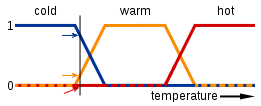
\includegraphics[width=0.38\textwidth]{fuzzyLogic}
            \end{center}
            \label{typical fuzzy logic}
            \caption{typical fuzzy logic}
        \end{figure}
        It's easy to see that the membership of y should be sense as a degree. But in the case of the numbers, no matter what series of them, could not be a continuous function or to be sense as degree. 
    \item Another way the evaluate that is to do the determination separately. We don't consider all of them but each of them once. That's to say, we evaluate a picture how it close it is to a typical character. For example, A '0' picture should be at least 90\% or higher when it was compared to a typical '0' picture and 10\% or lower compare to other numbers' picture. \\
        But still, how to evaluate this is a problem. The irony thing is, when I consider this in deep, I suddenly find out if a membership function like this was done, then we didn't need to implement the whole system because the task was completed.\\
\end{itemize}
Thus we actually need a simple way to evaluate and degreeize the membership function of y before we can actually walk into the next step.

\subsection{Applying Fuzzy Logic with BP Neural Network}
The main idea using BP Neural network is to minimize the cost, which means the difference between the hypothesis and the actual value. It takes these steps to do its job. 
\begin{itemize}
\item Step 1: Define the membership function, and get the subspace of fuzzy system.
\item Step 2: Define rules for the fuzzy learning system. \\
    Use $(x_1, x_2, y)$ as an example input, which can be set as (0.8, 0.4, 0.5). For instance, $M(x_1) = 0.3$, in area BZ, $M(x_2) = 0.4$, in area BD, $M(y) = 0.8$, in area 5, the relationship can be defined as $M(x_1) * M(x_2) * M(y)$(Note that though we use M(x) to represent membership function, they can be different function actually), which is $0.3 * 0.4 * 0.8 = 0.096$. Then we can say if BZ, BD, then 5. \\
    Suppose we had another input as (0.9, 0.2, 0.9), for instance, $M(x_1) = 0.5$, in area BZ, $M(x_2) = 0.5$, in area BD, $M(y) = 1$, in area 6, the relationship is $0.5 * 0.5 * 1 = 0.25$. Then we can say if BZ, BD, then 6. Here we got the same if but the different then. We choose the higher one for our conclusion, which means the "if BZ, BD, then 5" rule was discarded. \\
    Another thing worth mentioning is that usually there are two membership value of different subspaces in a given input, we also choose the higher one to use.
\item Step 3: Now we have already initial the network. We should train our network now. Our network had 5 layers. The first layer is input layer and the last layer is the output layer, which give our hypothesis. The second layer is the fuzzy layer, which takes our input and use membership function to compute it and give the pair of (value, subspace). The third layer was to use the rules we defined in the previous step and do the "and" operation. The fourth layer was to conclude the result done in the third layer. The last layer then was to analyse the conclusion from the forth layer.
    \begin{itemize}
        \item Since we use BP Neural Network to complete our task, we should first feedforward, and get the result of the current network.
        \item We compute the error of the fifth layer and give the differential of each parameter in layer four. Then we use the differential as gradient to do the batch gradient decent. Actually in each layer, we would do the gradient decent.
        \item When the error passed to the second layer, the whole network was freshed. We need to do a feedforward again and compute the error again. If it did not come down as expect, we repeat the step 3 again until the error decrease to a certain extend. 
    \end{itemize}
\end{itemize}
%------------------------------------------------

%\subsection{Subsection 2} % Sub-section

% Content

%----------------------------------------------------------------------------------------
%	CONCLUSION
%----------------------------------------------------------------------------------------

\section{Conclusion} % Major section

It's not hard to design a fuzzy learning system with BP Neural Network but the membership function for y is a huge problem, which prevent me from implement it into code. My future work was to consider and find a simple but effective the membership function for y. Once this was done, the training system can at once be completed. Actually, using BP Neural Network can be achieved a accuracy of 99.4\% now, and I hope doing it with fuzzy system can have a better result.


\newpage % Begins the essay on a new page instead of on the same page as the table of contents 

\section{Introduction to the Author}
I'm Luo WeiQiang, a year-4 student in Sun-Yet-Sun university. My student ID is 10389321. My major is software engineering. Now doing research in robotics in kinematics and machine learning in classifying data. 

\section{Explanation of the chosen idea}
I'm studying machine learning nowadays and just finish classifying the numerical characters in an accuracy of 99.4\%. Firstly I want to implement fuzzy learning system into my current project then I found out it was difficult in some problems. I would detail the problems in the following essay. Because there were a lot of projects coming I do not think I can finish it at last, so I wrote what I found out in these days and hope any feedback or advices for the current process. 

\newpage


%----------------------------------------------------------------------------------------
%	BIBLIOGRAPHY
%----------------------------------------------------------------------------------------

\begin{thebibliography}{1} % Bibliography - this is intentionally simple in this template

    \bibitem[1]{}
        Li-Xin Wang and Jerry M. Mendel (1992).
        \newblock Back-Propagation Fuzzy System as Nonlinear Dynamic System Identifiers
        \newblock {\em IEEE}, 92:1409--1416.


    \bibitem[2]{}
        Patrick K. Simpson (1992).
        \newblock Fuzzy Min-Max Neural Networks
        \newblock {\em IEEE}, 92:776--786.


    \bibitem[3]{}
        Toshinori Munakata, Yashvant Jani (1994).
        \newblock Fuzzy System An Overview
        \newblock {\em Communications of the ACM}, 37:69--76.


    \bibitem[4]{}
        Utpal Garain and Bidyut B. Chaudhuri (2002).
        \newblock Segmentation of Touching Characters in Printed Devnagari and Bangla Scripts Using Fuzzy Multifactorial Analysis
        \newblock {\em IEEE}, 02:449--459.


    \bibitem[5]{}
        Raghuraj Singh, C.S. Yadav, Prabhat Verma, Vibhash Yadav(2010)
        \newblock Optical Character Recognition (OCR) for Printed Devnagari Script Using Artificial Neural Network
        \newblock {\em International Journal of Computer Science \& Communication}, 01:91--95.

\end{thebibliography}
%----------------------------------------------------------------------------------------

\end{document}
